\chapter{Overview}
\label{cha:overview}


\section{Modeling concepts}

An {\opp} model consists of modules that communicate with message passing.
The active modules are termed \textit{simple modules}; they are written in C++,
using the simulation class library. Simple modules can be grouped into
\textit{compound modules} and so forth; the number of hierarchy levels is not
limited. Messages can be sent either via connections that span between
modules or directly to their destination modules. The concept of simple and
compound modules is similar to DEVS atomic and coupled models.
%TODO add ref to DEVS papers

Both simple and compound modules are instances of \textit{module types}.
When describing the model, the user defines module types; instances of these
module types serve as components for more complex module types. Finally,
the user creates the system module as a network module which is a special
compound module type without gates to the external world. When a module
type is used as a building block, there is no distinction whether it is a
simple or a compound module. This allows the user to transparently split a
module into several simple modules within a compound module, or do the
opposite, re-implement the functionality of a compound module in one simple
module, without affecting existing users of the module type.

In Fig. \ref{fig:ch-overview:modules}, boxes represent simple modules
(thick border) and compound modules (thin border).
Arrows connecting small boxes represent connections and gates.

\begin{figure}[htbp]
\begin{center}
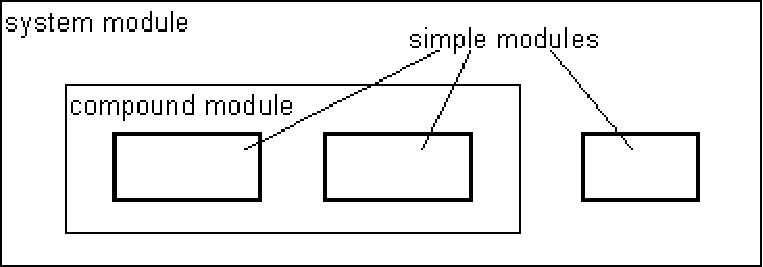
\includegraphics[width=3.772in, height=1.292in]{figures/usmanFig2}
\caption{Simple and compound modules}
\label{fig:ch-overview:modules}
\end{center}
\end{figure}


Modules communicate with messages which -- in addition to
usual attributes such as timestamp -- may contain arbitrary
data. Simple modules typically send messages via gates, but it is also
possible to send them directly to their destination modules. Gates are the
input and output interfaces of modules: messages are sent out through
output gates and arrive through input gates. An input and an output gate
can be linked with a connection. Connections are created within a single
level of module hierarchy: within a compound module, corresponding gates of
two submodules, or a gate of one submodule and a gate of the compound
module can be connected. Connections spanning across hierarchy levels are
not permitted, as it would hinder model reuse. Due to the hierarchical
structure of the model, messages typically travel through a chain of
connections, to start and arrive in simple modules. Compound modules act as
'cardboard boxes' in the model, transparently relaying messages between
their inside and the outside world. Properties such as propagation delay,
data rate and bit error rate, can be assigned to connections. One can also
define connection types with specific properties (termed channels) and
reuse them in several places. Modules can have parameters. Parameters are
mainly used to pass configuration data to simple modules, and to help
define model topology. Parameters may take string, numeric or boolean
values. Because parameters are represented as objects in the program,
parameters -- in addition to holding constants -- may transparently act as
sources of random numbers with the actual distributions provided with the
model configuration, they may interactively prompt the user for the value,
and they might also hold expressions referencing other parameters. Compound
modules may pass parameters or expressions of parameters to their
submodules.






{\opp} provides efficient tools for the user to describe the
structure of the actual system. Some of the main features are:
\begin{itemize}
\item{hierarchically nested modules}
\item{modules are instances of module types}
\item{modules communicate with messages through channels}
\item{flexible module parameters}
\item{topology description language}
\end{itemize}

\subsection{Hierarchical modules}


An {\opp} model consists of hierarchically nested
modules\index{module!hierarchy}, which communicate by passing
messages to each another.
{\opp} models are often referred to as \textit{networks}. The top
level module is the \textit{system module}.  The system module
contains \textit{submodules}, which can also contain submodules
themselves (Fig. \ref{fig:ch-overview:modules}). The depth of module
nesting is not limited; this allows the user to reflect the logical
structure of the actual system in the model structure.

Model structure is described in {\opp}'s NED language.

\begin{figure}[htbp]
\begin{center}
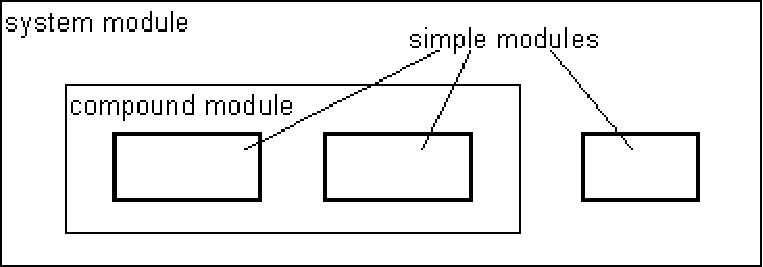
\includegraphics[width=3.772in, height=1.292in]{figures/usmanFig2}
\caption{Simple and compound modules}
\label{fig:ch-overview:modules}
\end{center}
\end{figure}


Modules that contain submodules are termed \textit{compound
  modules}\index{module!compound}, as opposed \textit{simple
  modules}\index{module!simple} which are at the lowest level of the
module hierarchy. Simple modules contain the algorithms in the model.
The user implements the simple modules in C++, using the {\opp}
simulation class library.


\subsection{Module types}
\index{module!types}

Both simple and compound modules are instances of \textit{module
  types}. While describing the model, the user defines module types;
instances of these module types serve as components for more complex
module types. Finally, the user creates the system module as an
instance of a previously defined module type; all modules of the
network are instantiated as submodules and sub-submodules of the
system module.

When a module type is used as a building block, there is no
distinction whether it is a simple or a compound module. This allows
the user to split a simple module into several
simple modules embedded into a compound\index{module!compound} module,
or vica versa, aggregate the functionality of a compound module into a
single simple module, without affecting existing users of the module
type.

Module types can be stored in files separately from the place
of their actual usage. This means that the user can group existing
module types and create \textit{component libraries}\index{module!libraries}. This feature
will be discussed later, in Chapter \ref{cha:run-sim}.



\subsection{Messages, gates, links}

Modules communicate by exchanging
\textit{messages}\index{message!exchanging}. In an actual simulation,
messages can represent frames or packets in a computer network, jobs
or customers in a queuing network or other types of mobile entities.
Messages can contain arbitrarily complex data structures. Simple
modules can send messages either directly to their destination or
along a predefined path, through gates and connections.


The ``local simulation time'' of a module advances when the module
receives a message. The message can arrive from another module
or from the same module (\textit{self-messages} are used to implement
timers).


\textit{Gates}\index{gate} are the input and output interfaces of
modules; messages are sent out through output gates and arrive through
input gates.

Each \textit{connection}\index{connection} (also called
\textit{link}\index{link}) is created within a single level of the
module hierarchy: within a compound module, one can connect the
corresponding gates of two submodules, or a gate of one submodule and
a gate of the compound module (Fig.
\ref{fig:ch-overview:connections}).

\begin{figure}[htbp]
\begin{center}
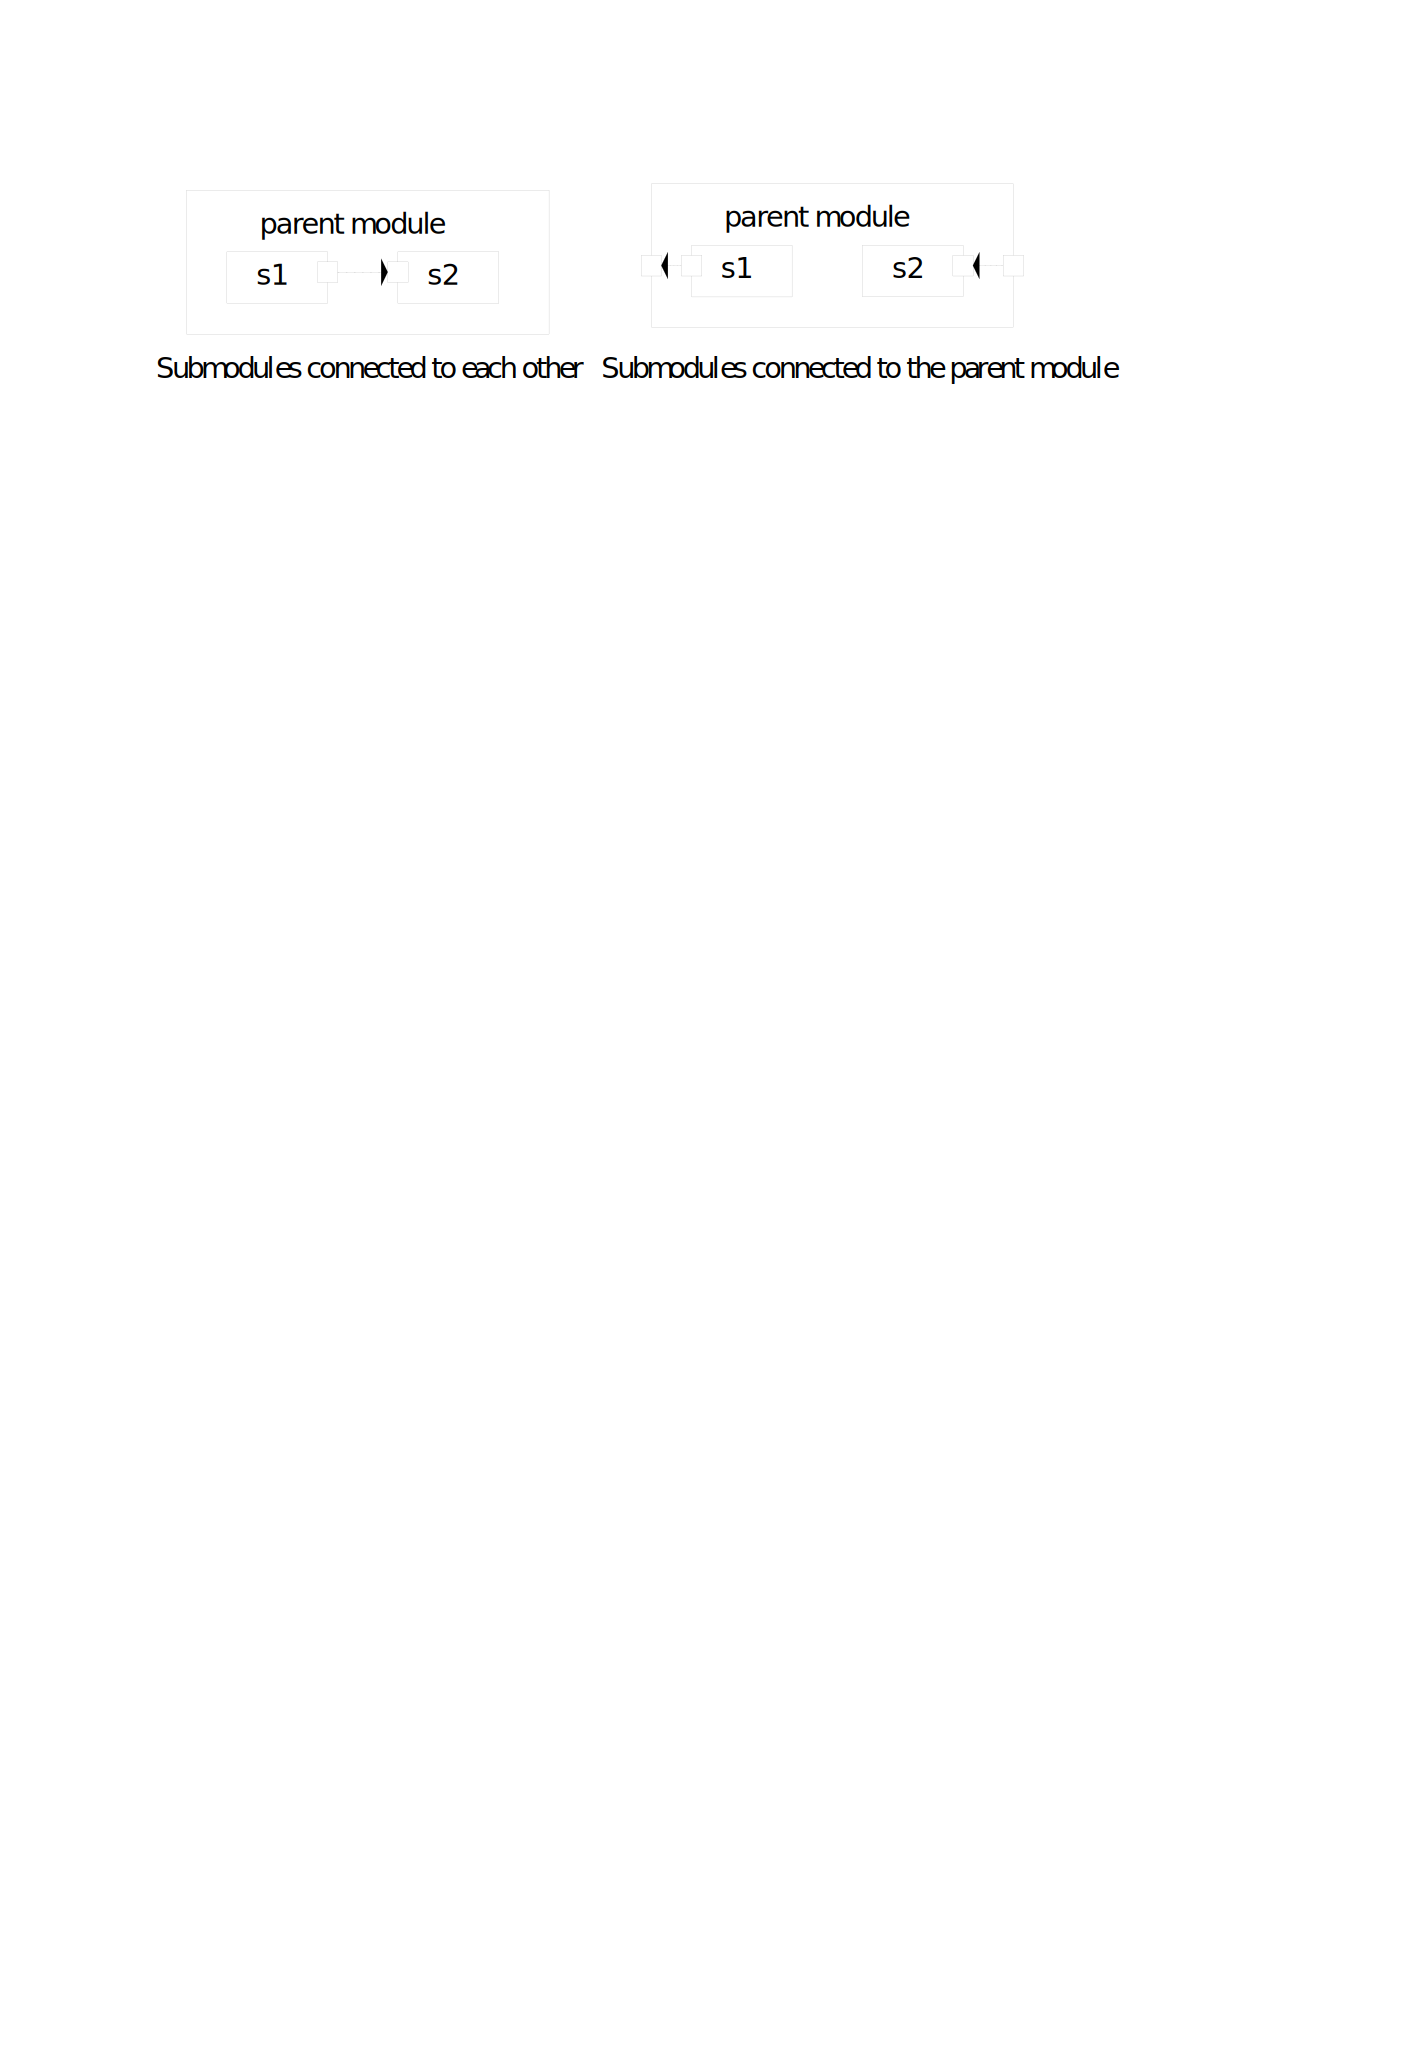
\includegraphics[width=5.061in, height=1.121in]{figures/usmanFig3}
\caption{Connections}
\label{fig:ch-overview:connections}
\end{center}
\end{figure}

Due to the hierarchical structure of the model, messages typically
travel through a series of connections, to start and arrive in simple
modules. Such series of connections that go from simple module to
simple module are called \textit{routes}.  Compound modules act as
`cardboard boxes' in the model, transparently relaying messages
between their inside and the outside world.


\subsection{Modeling of packet transmissions}

Connections can be assigned three parameters, which facilitate
the modeling of communication networks, but can be useful in
other models too: \textit{propagation delay}, \textit{bit error rate}
and \textit{data rate}, all three being optional. One can specify
link parameters individually for each connection, or define link types
and use them throughout the whole model.

Propagation delay is the amount of time the arrival of
the message is delayed by when it travels through the channel.

Bit error rate speficifies the probability that a bit is incorrectly
transmitted, and allows for simple noisy channel modelling.

Data rate is specified in bits/second, and it is used for calculating
transmission time of a packet.

When data rates are in use, the sending of the message in the model
corresponds to the transmission of the first bit, and
the arrival of the message corresponds to the reception
of the last bit. This model is not always applicable,
for example protocols like Token Ring and FDDI do not wait
for the frame to arrive in its entirety, but rather start repeating
its first bits soon after they arrive -- in other words,
frames ``flow through'' the stations, being delayed only a few bits.
If you want to model such networks, the data rate modeling feature
of {\opp} cannot be used.



\subsection{Parameters}
\index{module!parameters}
\index{parameters|see{module parameters}}

Modules can have parameters. Parameters can be assigned either
in the NED files or the configuration file omnetpp.ini.

Parameters may be used to customize simple module behaviour,
and for parameterizing the model topology.

Parameters can take string, numeric or boolean values, or can
contain XML data trees. Numeric values include expressions using
other parameters and calling C functions, random variables from
different distributions, and values input interactively by the user.

Numeric-valued parameters can be used to construct topologies in a
flexible way. Within a compound module, parameters can define the
number of submodules, number of gates, and the way the internal
connections are made.


\subsection{Topology description method}
\index{topology!description}
The user defines the structure of the model in NED language descriptions
(Network Description).The NED language will be discussed in detail
in Chapter \ref{cha:the-ned-language}.


\section{Programming the algorithms}

The simple\index{module!simple} modules of a model contain algorithms
as C++ functions.
The full flexibility and power of the programming language can
be used, supported by the {\opp} simulation class library.
The simulation programmer can choose between event-driven and process-style
description, and can freely use object-oriented concepts
(inheritance, polymorphism etc) and design patterns to extend the
functionality of the simulator.

Simulation objects (messages, modules, queues etc.) are represented
by C++ classes. They have been designed to work together efficiently,
creating a powerful simulation programming framework.
The following classes are part of the simulation class library:

\begin{itemize}
  \item{modules, gates, connections etc.}
  \item{parameters}
  \item{messages}
  \item{container classes (e.g. queue, array)}
  \item{data collection classes}
  \item{statistic and distribution estimation classes (histograms, $P^2$
  algorithm for calculating quantiles etc.)}
  \item{transient detection and result accuracy detection classes}
\end{itemize}

The classes are also specially instrumented, allowing one
to traverse objects of a running simulation and display information
about them such as name, class name, state variables or contents.
This feature has made it possible to create a simulation GUI where
all internals of the simulation are visible.


% \subsection{Creating simple modules}
% \index{module!simple!creation}
%
% Each simple\index{module!simple} module type is implemented with a C++ class. Simple
% module classes are derived from a simple module base class, by
% redefining the virtual function that contains the algorithm.
% The user can add other member functions to the class to split
% up a complex algorithm; he can also add data members to the class.
%
% It is also possible to derive new simple\index{module!simple} module classes from
% existing ones. For example, if one wants to experiment with retransmission
% timeout schemes in a transport protocol, he can implement the
% protocol in one class, create a virtual function for the retransmission
% algorithm and then derive a family of classes that implement
% concrete schemes. This concept is further supported by the fact
% that in the network description, actual module types can be parameters.
%
%
% \subsection{Object mechanisms}
%
% The use of smart container classes allows the user to build
% \textit{aggregate data structures}\index{aggregate data structures}.
% For example, one can add any number of objects to a message object as
% parameters. Since the added objects can contain further objects,
% complex data structures can be built.
%
% There is an efficient \textit{ownership}\index{ownership} mechanism
% built in. The user can specify an owner for each object; then, the
% owner object will have the responsibility of destroying that object.
% Most of the time, the ownership mechanism works transparently;
% ownership only needs to be explicitly managed when the user wants to
% do something non-typical.
%
%
% The \textit{foreach}\index{forEachChild mechanism} mechanism allows one to
% enumerate the objects inside a container object in a uniform way and
% do some operation on them. This feature which makes it possible to
% handle many objects together. (The \textit{foreach} feature is extensively used
% by the user interfaces with debugging capability and the snapshot
% mechanism; see later.)
%
%
% \subsection{Derive new classes}
%
% It most cases, the functionality offered by the {\opp} classes
% is enough for the user. But if it is needed, one can derive new
% classes from the existing ones or create entirely new classes.
% For flexibility, several member functions are declared virtual.
% When the user creates new classes, certain rules need to be kept
% so that the object can fully work together with other objects.
%
%
% \subsection{Self-describing objects to ease debugging}
% \index{debugging}
%
%
%
% A unique feature called \textit{snapshot}\index{snapshot} allows the
% user to dump the contents of the simulation model or a part of it into
% a text file. The file will contain textual reports about every object;
% this can be of invaluable help at times of debugging. Ordinary
% variables can also be made to appear in the snapshot file. Snapshot
% creations can be scheduled from within the simulation program or done
% from the user interface.
%


\section{Using {\opp}}


\subsection{Building and running simulations}
\index{simulation!building}
\index{simulation!running}

This section provides insight into working with {\opp} in practice:
Issues such as model files, compiling and running simulations are
discussed.

An {\opp} model consists of the following parts:
\begin{itemize}
  \item{NED language topology description(s)\index{ned!files} (\texttt{.ned} files)
    which describe the module structure with parameters, gates etc.
    NED files can be written using any text editor or the
    GNED graphical editor\index{ned!graphical editor}.}
  \item{Message definitions (\texttt{.msg} files). You can define various message
    types and add data fields to them. {\opp} will translate message definitions
    into full-fledged C++ classes.}
  \item{Simple modules sources. They are C++ files, with \texttt{.h}/\texttt{.cc} suffix.}
\end{itemize}

The simulation system provides the following components:
\begin{itemize}
  \item{Simulation kernel\index{simulation!kernel}. This contains the
    code that manages the simulation and the simulation class library.
    It is written in C++, compiled and put together to form a library
    (a file with .a or .lib extension)}
  \item{User interfaces\index{simulation!user interface}.
    \index{user interface} {\opp} user interfaces
    are used in simulation execution, to facilitate debugging,
    demonstration, or batch execution of simulations. There are
    several user interfaces, written in C++, compiled and put together
    into libraries (\texttt{.a} or \texttt{.lib} files).}
\end{itemize}


Simulation programs are built from the above components. First,
\ttt{.msg} files are translated into C++ code using the \ttt{opp\_msgc}.
program. Then all C++ sources are compiled, and linked with the simulation
kernel and a user interface library to form a simulation executable.
NED files\index{ned!files} can either be also translated into C++
(using \ttt{nedtool}) and linked in, or loaded dynamically in their original
text forms when the simulation program starts.



\subsubsection{Running the simulation and analyzing the results}

The simulation executable is a standalone program,
thus it can be run on other machines without {\opp} or the model files
being present. When the program is started, it reads a configuration
file\index{simulation!configuration file} (usually called
\texttt{omnetpp.ini}\index{omnetpp.ini}). This file contains settings that
control how the simulation is executed, values for model parameters, etc.
The configuration file can also prescribe several simulation runs; in
the simplest case, they will be executed by the simulation program one
after another.

The output of the simulation is written into data files: output vector
files\index{output!vector file}, output scalar files
\index{output!scalar file}, and possibly the user's own output files.
{\opp} provides a GUI tool named Plove to view and plot the contents
of output vector files. It is not expected that someone will
process the result files using {\opp} alone: output files are text
files in a format which can be read into math packages like Matlab
or Octave, or imported into spreadsheets like OpenOffice Calc,
Gnumeric or MS Excel (some preprocessing using \fprog{sed}, \fprog{awk}
or \fprog{perl} might be required, this will be discussed later).
All these external programs provide rich functionality for statistical
analysis and visualization, and it is outside the scope of {\opp} to
duplicate their efforts. This manual briefly describes
some data plotting programs and how to use them with {\opp}.

Output scalar files can be visualized using the Scalars tool.
It can draw bar charts, x-y plots (e.g. throughput vs offered load),
or export data via the clipboard for more detailed analysis into
spreadsheets and other programs.


\subsubsection{User interfaces}
\index{simulation!user interface}

The primary purpose of user interfaces is to make the internals
of the model visible to the user, to control simulation execution,
and possibly allow the user to intervene by changing variables/objects
inside the model. This is very important in the development/debugging
phase of the simulation project. Just as important, a hands-on
experience allows the user to get a `feel' of the model's
behaviour. The graphical user interface can also be used to
demonstrate a model's operation.


The same simulation model can be executed with different user
interfaces, without any change in the model files themselves.
The user would test and debug the simulation with a powerful
graphical user interface, and finally run it with a simple and
fast user interface that supports batch execution.


\subsubsection{Component libraries}
\index{module!libraries}

Module types can be stored in files separate from the place
of their actual use. This enables the user to group existing
module types and create component libraries.


\subsubsection{Universal standalone simulation programs}


A simulation executable can store several independent models
that use the same set of simple modules. The user can specify
in the configuration file which model is to be run. This
allows one to build one large executable that contains several
simulation models, and distribute it as a standalone simulation
tool. The flexibility of the topology description language also
supports this approach.


\subsection{What is in the distribution}

If you installed the source distribution, the omnetpp directory on your system
should contain the following subdirectories. (If you installed a precompiled
distribution, some of the directories may be missing, or there might be
additional directories, e.g. containing software bundled with {\opp}.)

The simulation system itself:

\begin{Verbatim}[commandchars=\\\{\}]
  \tbf{omnetpp/}         {\opp} root directory
    \tbf{bin/}           {\opp} executables (GNED, nedtool, etc.)
    \tbf{include/}       header files for simulation models
    \tbf{lib/}           library files
    \tbf{bitmaps/}       icons that can be used in network graphics
    \tbf{doc/}           manual (PDF), readme, license, etc.
      \tbf{manual/}      manual in HTML
      \tbf{tictoc-tutorial/}  introduction into using {\opp}
      \tbf{api/}         API reference in HTML
      \tbf{nedxml-api/}  API reference for the NEDXML library
      \tbf{src/}         sources of the documentation
    \tbf{src/}           {\opp} sources
      \tbf{nedc/}        nedtool, message compiler
      \tbf{sim/}         simulation kernel
        \tbf{parsim/}    files for distributed execution
        \tbf{netbuilder/}files for dynamically reading NED files
      \tbf{envir/}       common code for user interfaces
      \tbf{cmdenv/}      command-line user interface
      \tbf{tkenv/}       Tcl/Tk-based user interface
      \tbf{gned/}        graphical NED editor
      \tbf{plove/}       output vector analyzer and plotting tool
      \tbf{scalars}      output scalar analyzer and plotting tool
      \tbf{nedxml/}      NEDXML library
      \tbf{utils/}       makefile-creator, documentation tool, etc.
    \tbf{test/}          regression test suite
      \tbf{core/}        regression test suite for the simulation library
      \tbf{distrib/}     regression test suite for built-in distributions
      ...
\end{Verbatim}

Sample simulations are in the \texttt{samples} directory.

\begin{Verbatim}[commandchars=\\\{\}]
    \tbf{samples/}     directories for sample simulations
      \tbf{aloha/}     models the Aloha protocol
      \tbf{cqn/}       Closed Queueing Network
      ...
\end{Verbatim}

The \texttt{contrib} directory contains material from the {\opp} community.

\begin{Verbatim}[commandchars=\\\{\}]
    \tbf{contrib/}     directory for contributed material
      \tbf{octave/}    Octave scripts for result processing
      \tbf{emacs/}     NED syntax highlight for Emacs
\end{Verbatim}

You may also find additional directories like \texttt{msvc/}, which contain
integration components for Microsoft Visual C++, etc.


%%% Local Variables:
%%% mode: latex
%%% TeX-master: "usman"
%%% End:
